\documentclass[12pt]{article}

\usepackage{algorithm}
\usepackage{algorithmicx}
\usepackage{algpseudocode}
\usepackage{amsmath}
\usepackage{amsthm}
\usepackage{tikz}
\usetikzlibrary{arrows,automata}

\title{EECS 477 HW3}
\author{Andrew Mason}

\begin{document}
\maketitle

\begin{enumerate}
    % #1
    \item
        I originally thought to model this as a variation of the matrix
        rounding problem discussed in class, but this has the unfortunate
        result of actually maximizing the number of nurses assigned to each
        shift/department pair.

        Instead, if we start by assigning the maximum number of nurses allowed
        to each shift/department pair, we can formulate another variation of
        the matrix rounding problem which attempts to maximize the number of
        nurses witheld from each shift/department pair. The edges incident on
        the ``matrix nodes'' (the nodes representing each shift/department
        pair) each have $l_{ij},u_{ij}=0,d$, where $d$ is the difference
        between the lower and upper bounds for that node in the original
        matrix. The column nodes then have $l_{ij},u_{ij}=0, d_c$, where $d_c$
        is the difference between the column lower bound in the original
        matrix, and the sum of the upper bounds for each matrix node in the
        original matrix. The row nodes similarly have $l_{ij},u_{ij}=0,d_r$.

        So, our network looks like:
        \begin{center}
            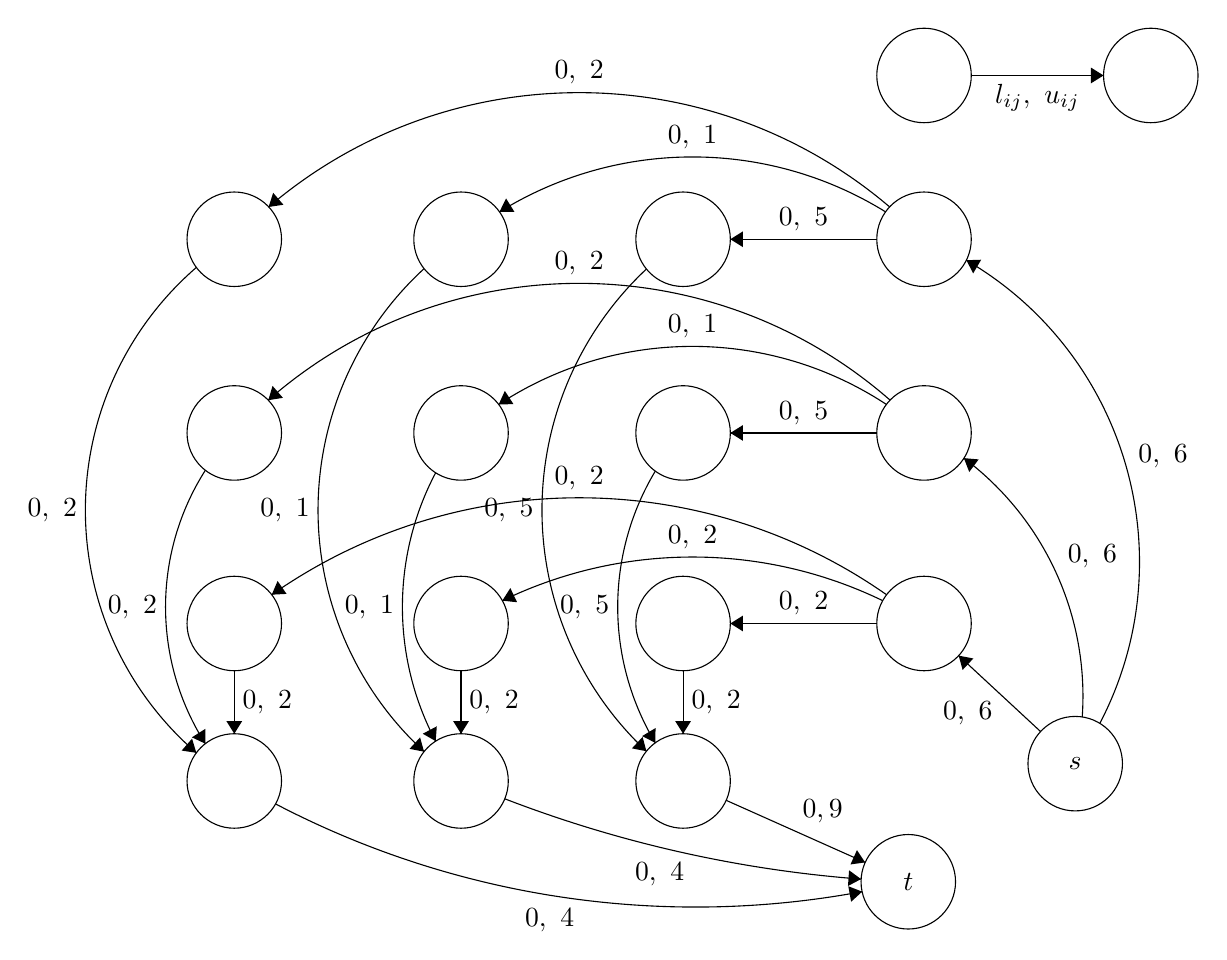
\begin{tikzpicture}[scale=0.2]
                \tikzstyle{every node}+=[inner sep=0pt]
                \draw [black] (56.5,-4) circle (3);
                \draw [black] (70.9,-4) circle (3);
                \draw [black] (12.7,-14.4) circle (3);
                \draw [black] (27.1,-14.4) circle (3);
                \draw [black] (41.2,-14.4) circle (3);
                \draw [black] (56.5,-14.4) circle (3);
                \draw [black] (12.7,-26.7) circle (3);
                \draw [black] (27.1,-26.7) circle (3);
                \draw [black] (41.2,-26.7) circle (3);
                \draw [black] (56.5,-26.7) circle (3);
                \draw [black] (12.7,-38.8) circle (3);
                \draw [black] (27.1,-38.8) circle (3);
                \draw [black] (41.2,-38.8) circle (3);
                \draw [black] (56.5,-38.8) circle (3);
                \draw [black] (12.7,-48.8) circle (3);
                \draw [black] (27.1,-48.8) circle (3);
                \draw [black] (41.2,-48.8) circle (3);
                \draw [black] (55.5,-55.2) circle (3);
                \draw (55.5,-55.2) node {$t$};
                \draw [black] (66.1,-47.7) circle (3);
                \draw (66.1,-47.7) node {$s$};
                \draw [black] (59.5,-4) -- (67.9,-4);
                \fill [black] (67.9,-4) -- (67.1,-3.5) -- (67.1,-4.5);
                \draw (63.7,-4.5) node [below] {$l_{ij},\mbox{ }u_{ij}$};
                \draw [black] (59.185,-15.733) arc (59.72274:-27.55944:22.175);
                \fill [black] (59.19,-15.73) -- (59.62,-16.57) -- (60.13,-15.7);
                \draw (70.08,-28.17) node [right] {$0,\mbox{ }6$};
                \draw [black] (59.033,-28.302) arc (53.13091:-3.99657:18.896);
                \fill [black] (59.03,-28.3) -- (59.37,-29.18) -- (59.97,-28.38);
                \draw (65.6,-34.54) node [right] {$0,\mbox{ }6$};
                \draw [black] (63.9,-45.66) -- (58.7,-40.84);
                \fill [black] (58.7,-40.84) -- (58.95,-41.75) -- (59.63,-41.02);
                \draw (59.28,-43.74) node [below] {$0,\mbox{ }6$};
                \draw [black] (53.5,-14.4) -- (44.2,-14.4);
                \fill [black] (44.2,-14.4) -- (45,-14.9) -- (45,-13.9);
                \draw (48.85,-13.9) node [above] {$0,\mbox{ }5$};
                \draw [black] (29.542,-12.661) arc (121.76626:58.23374:23.284);
                \fill [black] (29.54,-12.66) -- (30.49,-12.66) -- (29.96,-11.81);
                \draw (41.8,-8.67) node [above] {$0,\mbox{ }1$};
                \draw [black] (14.885,-12.346) arc (130.41235:49.58765:30.412);
                \fill [black] (14.88,-12.35) -- (15.82,-12.21) -- (15.17,-11.45);
                \draw (34.6,-4.59) node [above] {$0,\mbox{ }2$};
                \draw [black] (53.5,-26.7) -- (44.2,-26.7);
                \fill [black] (44.2,-26.7) -- (45,-27.2) -- (45,-26.2);
                \draw (48.85,-26.2) node [above] {$0,\mbox{ }5$};
                \draw [black] (29.489,-24.889) arc (123.33513:56.66487:22.403);
                \fill [black] (29.49,-24.89) -- (30.43,-24.87) -- (29.88,-24.03);
                \draw (41.8,-20.7) node [above] {$0,\mbox{ }1$};
                \draw [black] (14.856,-24.615) arc (131.17311:48.82689:29.991);
                \fill [black] (14.86,-24.62) -- (15.79,-24.47) -- (15.13,-23.71);
                \draw (34.6,-16.7) node [above] {$0,\mbox{ }2$};
                \draw [black] (53.5,-38.8) -- (44.2,-38.8);
                \fill [black] (44.2,-38.8) -- (45,-39.3) -- (45,-38.3);
                \draw (48.85,-38.3) node [above] {$0,\mbox{ }2$};
                \draw [black] (29.724,-37.349) arc (115.84349:64.15651:27.703);
                \fill [black] (29.72,-37.35) -- (30.66,-37.45) -- (30.23,-36.55);
                \draw (41.8,-34.08) node [above] {$0,\mbox{ }2$};
                \draw [black] (15.078,-36.973) arc (125.01248:54.98752:34.025);
                \fill [black] (15.08,-36.97) -- (16.02,-36.92) -- (15.45,-36.1);
                \draw (34.6,-30.32) node [above] {$0,\mbox{ }2$};
                \draw [black] (12.7,-41.8) -- (12.7,-45.8);
                \fill [black] (12.7,-45.8) -- (13.2,-45) -- (12.2,-45);
                \draw (13.2,-43.8) node [right] {$0,\mbox{ }2$};
                \draw [black] (27.1,-41.8) -- (27.1,-45.8);
                \fill [black] (27.1,-45.8) -- (27.6,-45) -- (26.6,-45);
                \draw (27.6,-43.8) node [right] {$0,\mbox{ }2$};
                \draw [black] (41.2,-41.8) -- (41.2,-45.8);
                \fill [black] (41.2,-45.8) -- (41.7,-45) -- (40.7,-45);
                \draw (41.7,-43.8) node [right] {$0,\mbox{ }2$};
                \draw [black] (43.94,-50.03) -- (52.76,-53.97);
                \fill [black] (52.76,-53.97) -- (52.24,-53.19) -- (51.83,-54.1);
                \draw (50.06,-51.48) node [above] {$0,9$};
                \draw [black] (52.505,-55.031) arc (-94.31889:-111.08028:79.568);
                \fill [black] (52.5,-55.03) -- (51.74,-54.47) -- (51.67,-55.47);
                \draw (39.71,-53.97) node [below] {$0,\mbox{ }4$};
                \draw [black] (52.567,-55.827) arc (-79.41981:-117.58934:57.589);
                \fill [black] (52.57,-55.83) -- (51.69,-55.48) -- (51.87,-56.47);
                \draw (32.73,-56.86) node [below] {$0,\mbox{ }4$};
                \draw [black] (10.864,-46.433) arc (-147.51999:-212.48001:16.169);
                \fill [black] (10.86,-46.43) -- (10.86,-45.49) -- (10.01,-46.03);
                \draw (7.83,-37.75) node [left] {$0,\mbox{ }2$};
                \draw [black] (25.488,-46.274) arc (-152.16764:-207.83236:18.257);
                \fill [black] (25.49,-46.27) -- (25.56,-45.33) -- (24.67,-45.8);
                \draw (22.88,-37.75) node [left] {$0,\mbox{ }1$};
                \draw [black] (39.436,-46.378) arc (-149.04755:-210.95245:16.776);
                \fill [black] (39.44,-46.38) -- (39.45,-45.44) -- (38.6,-45.95);
                \draw (36.55,-37.75) node [left] {$0,\mbox{ }5$};
                \draw [black] (10.294,-47.012) arc (-130.83998:-229.16002:20.372);
                \fill [black] (10.29,-47.01) -- (10.02,-46.11) -- (9.36,-46.87);
                \draw (2.74,-31.6) node [left] {$0,\mbox{ }2$};
                \draw [black] (24.753,-46.936) arc (-132.58201:-227.41799:20.828);
                \fill [black] (24.75,-46.94) -- (24.5,-46.03) -- (23.83,-46.76);
                \draw (17.52,-31.6) node [left] {$0,\mbox{ }1$};
                \draw [black] (38.872,-46.911) arc (-133.15246:-226.84754:20.988);
                \fill [black] (38.87,-46.91) -- (38.63,-46) -- (37.95,-46.73);
                \draw (31.74,-31.6) node [left] {$0,\mbox{ }5$};
            \end{tikzpicture}
        \end{center}

        And this can now be solved by max flow.\\
    % #2
    \item
    % #3
    \item
    % #4
    \item Omitted.\\
    % #5
    \item
    % #6
    \item Postponed.\\
    % #7
    \item
    % #8
    \item Postponed.\\
\end{enumerate}
\end{document}
